\subsection{Virtual Function II}
The figures below are depicting the axis plots of the virtual hyperparameter space function II to be optimized with the available hyppopy solvers. 
\begin{figure}[h]
	\begin{subfigure}{0.32\textwidth}
		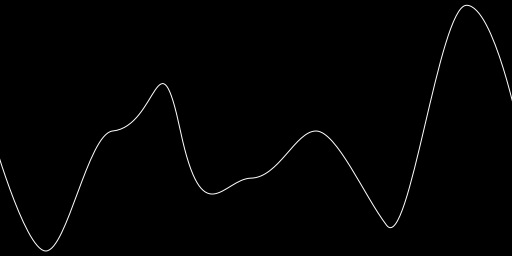
\includegraphics[width=\linewidth]{gt_II/axis_00} 
		\caption{axis 00}
		\label{fig:axis00_II}
	\end{subfigure}
	\begin{subfigure}{0.32\textwidth}
		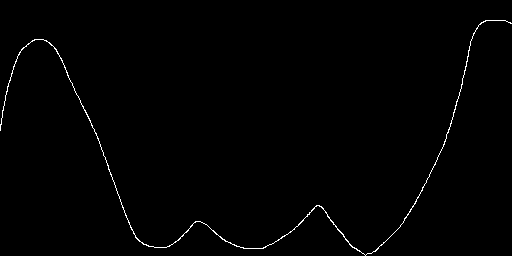
\includegraphics[width=\linewidth]{gt_II/axis_01}
		\caption{axis 01}
		\label{fig:axis01_II}
	\end{subfigure}
	\begin{subfigure}{0.32\textwidth}
		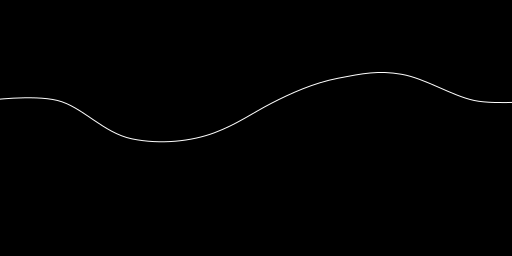
\includegraphics[width=\linewidth]{gt_II/axis_02}
		\caption{axis 02}
		\label{fig:axis02_II}
	\end{subfigure}
\end{figure}

\begin{figure}[h]
	\begin{subfigure}{0.32\textwidth}
		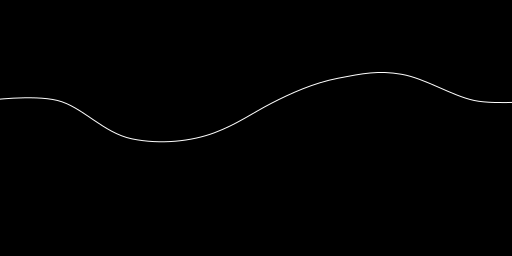
\includegraphics[width=\linewidth]{gt_II/axis_03} 
		\caption{axis 03}
		\label{fig:axis03_II}
	\end{subfigure}
	\begin{subfigure}{0.32\textwidth}
		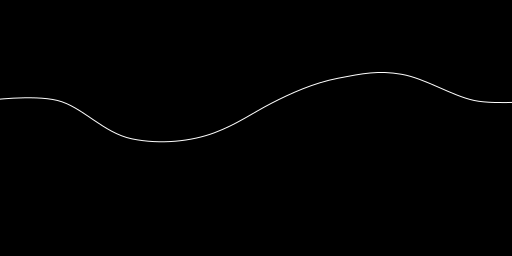
\includegraphics[width=\linewidth]{gt_II/axis_04}
		\caption{axis 04}
		\label{fig:axis04_II}
	\end{subfigure}
	\begin{subfigure}{0.32\textwidth}
		
\includegraphics[width=\linewidth]{gt_II/dummy}
		\caption{}
		\label{fig:dummy1_II}
	\end{subfigure}
\end{figure}


\newpage


\subsubsection{Minimum Finding Abilities}

The pictures below depict the accuracies reached on the individual axis. The light green region is the ground truth and the red, blue, violet and orange lines are the results after 50, 100, 250, and 500 iterations. Each line is the mean result over 50 individual optimizations on the target function.

\begin{figure}[h]
	\begin{subfigure}{0.5\textwidth}
		\includegraphics[width=0.9\linewidth]{data_II/hyperopt_deviation}
		\label{fig:hyperopt_deviation_II}
	\end{subfigure}
	\begin{subfigure}{0.5\textwidth}
		\includegraphics[width=0.9\linewidth]{data_II/optunity_deviation}
		\label{fig:optunity_deviation_II}
	\end{subfigure}
\end{figure}

\begin{figure}[h]
	\begin{subfigure}{0.5\textwidth}
		\includegraphics[width=0.9\linewidth]{data_II/optuna_deviation} 
		\label{fig:optuna_deviation_II}
	\end{subfigure}
	\begin{subfigure}{0.5\textwidth}
		\includegraphics[width=0.9\linewidth]{data_II/randomsearch_deviation}
		\label{fig:randomsearch_deviation_II}
	\end{subfigure}
\end{figure}

\begin{figure}[h]
	\begin{subfigure}{0.5\textwidth}
		\includegraphics[width=0.9\linewidth]{data_II/quasirandomsearch_deviation} 
		\label{fig:quasirandomsearch_deviation_II}
	\end{subfigure}
	\begin{subfigure}{0.5\textwidth}
		
\includegraphics[width=0.9\linewidth]{data_II/dummy}
		\label{fig:dummy2_II}
	\end{subfigure}
\end{figure}


\newpage


\subsubsection{Relative Distances to the Axis Optima}

The pictures in this section depict the mean distance and the standard deviation per axis for each solver.

\begin{figure}[h]
	\begin{subfigure}{0.5\textwidth}
		\includegraphics[width=0.9\linewidth]{data_II/errorbars_50}
		\label{fig:errorbars_50_II}
	\end{subfigure}
	\begin{subfigure}{0.5\textwidth}
		\includegraphics[width=0.9\linewidth]{data_II/errorbars_100}
		\label{fig:errorbars_100_II}
	\end{subfigure}
\end{figure}

\begin{figure}[h]
	\begin{subfigure}{0.5\textwidth}
		\includegraphics[width=0.9\linewidth]{data_II/errorbars_250}
		\label{fig:errorbars_250_II}
	\end{subfigure}
	\begin{subfigure}{0.5\textwidth}
		\includegraphics[width=0.9\linewidth]{data_II/errorbars_500}
		\label{fig:errorbars_500_II}
	\end{subfigure}
\end{figure}


\newpage


\subsubsection{Convergence Beahviour}

The pictures in this section depict the loss over iteration plots for each of the 50 iterations for each solver. For better visualization the Loss values are sorted, so the mapping between Iteration and Loss values might not be correct. The purpose of these plots is to show the overall Loss curve for each solver and it's variation over different runs.  

\begin{figure}[h]
	\begin{subfigure}{0.5\textwidth}
		\includegraphics[width=0.9\linewidth]{data_II/losshistory_50}
		\label{fig:losshistory_50_II}
	\end{subfigure}
	\begin{subfigure}{0.5\textwidth}
		\includegraphics[width=0.9\linewidth]{data_II/losshistory_100}
		\label{fig:losshistory_100_II}
	\end{subfigure}
\end{figure}

\begin{figure}[h]
	\begin{subfigure}{0.5\textwidth}
		\includegraphics[width=0.9\linewidth]{data_II/losshistory_250}
		\label{fig:losshistory_250_II}
	\end{subfigure}
	\begin{subfigure}{0.5\textwidth}
		\includegraphics[width=0.9\linewidth]{data_II/losshistory_500}
		\label{fig:losshistory_500_II}
	\end{subfigure}
\end{figure}